\title{A topological characterisation of the affine plane as an algebraic variety}\label{art8}
\markright{A topological characterisation of the affine plane as an algebraic variety}

\author{By~ C.P. Ramanujam\footnote{This work was done when the author was at the Tata Institute of Fundamental Research.}}
\markboth{C.P. Ramanujam}{A topological characterisation of the affine plane as an algebraic variety}

\date{}
\maketitle

\setcounter{page}{97}

\section{Statement of results}\label{art8-sec1}%% 1

\setcounter{pageoriginal}{74}
This\pageoriginale  investigation arose from an attempt to answer the following question, raised by M. P. Murthy: If $X$ is an affine algebraic variety over a field $k$ such that $X \times A^1 \approx A^3$, where $A^n$ denotes the affine $n$-space over $k$, is $X$ isomorphic to $A^2$? It was hoped that when $k=C$, just the hypothesis that $X$ is a non-singular, affine, rational and contractible surface would imply that $X \approx \mathbb{C}^2$. This, however, is not true as we show by a counter-example. We are unable to decide if the variety $Y$ of this counter-example also satisfies the condition $Y \times \mathbb{C} \approx \mathbb{C}^3$.\footnote{Examples of compact 4-manifolds with boundary which are contractible and whose boundary is a homology 3-sphere but not a homotopy sphere have been given by several authors (Mazur, Poinereau, -----). Our counter-example also provides another such.}

On the other hand, we do prove the following positive result.

\begin{theorem*}
Let $X$ be a non-singular complex algebraic surface which is contractible AND simply connected at infinity. Then $X$ is isomorphic to the affine two-space as an algebraic variety.
\end{theorem*}

The idea of the proof is to embed $X$ as a Zariski open subset of a complete non-singular surface such that the complement is a union of non-singular curves with normal crossings, and to use the contractibility and simple-connectedness at infinity of $X$ to work out the geometric configuration of these curves. We prove that after suitable transformations, we are reduced to the case where the complement consists of a single non-singular curve, from which it follows easily that the compactification is the projective plane and the curve a line.

We shall first prove the theorem, and then proceed to give the counter example. The methods of the proof of the theorem are analogous to those of Mumford \cite{art8-key2}.

\section{Proof of the theorem}\label{art8-sec2}%% 2
Let $X$ be as in the statement of the theorem. By the Nagata compactification\pageoriginale  theorem \cite{art8-key3} and the theorem of resolution of singularities of an algebraic surface \cite{art8-key1}, we may assume $X$ embedded as a Zariski open subset of a complete non-singular (hence projective, see \cite{art8-key4}) surface $\bar{X}$, such that if $\bar{X} - X = Y$ and $Y_i (1 \leqq i \leqq n)$ are the components of $Y$, each $Y_i$ is a complete non-singular curve, and we have  the following further conditions:
\begin{itemize}
\item[(i)] For two distinct indices $i, j$, either $Y_i \bigcap Y_j = \oslash$ or $Y_i \bigcap Y_j$ consists of a single point where $Y_i$ and $Y_j$ meet transversally.   

\item[(ii)] For three distinct indices $i,j,k$, $Y_i \bigcap Y_j \bigcap Y_k = \oslash$.

The contractibility of $X$ implies some further conditions. In fact, by Poincar\'e duality on $X$, we get\footnote{All homologies and cohomologies have integral coefficients, unless otherwise indicated. Cohomology with compact supports is denoted by $H^*_c$.}
\begin{equation*}
H^i (\bar{X}, Y) \approx H^i_c (X) \approx H_{4-i} (X) \approx 
\left\{
\begin{aligned}
0 & \text{ \quad if~ } i < 4\\
Z & \text{ \quad if~ } i = 4,
\end{aligned}
\right.
\end{equation*}
so that by the cohomology exact sequence, we have isomorphisms
$$
H^i (\bar{X}) \approx H^i (Y), \qquad 0 \leqq i \leqq 3.
$$
Hence $Y$ is connected, $H^2 (\bar{X}) \to H^2 (Y)$ is an isomorphism and $H^3 (\bar{X}) =0$. By duality, $H_1 (\bar{X}) =0$, hence also $H^1(Y) =0$. From this, we deduce the following three conditions:

\item[(iii)] Any two components $Y_i$, $Y_j$ can be joined by a chain $Y_i = Y_{i_1}$, $Y_{i_2}, \ldots, Y_{i_p} = Y_j$ such that $Y_{i_k} \cap Y_{i_{k+1}} \neq \oslash$, $1 \leqq k \leqq p -1$.

\item[(iv)] There is no chain of components $Y_{i_1} , \ldots, Y_{i_p} (p \leqq 3)$ such that $Y_{i_k} \cap Y_{i_{k+1}} \neq \oslash$, $1 \leqq k\leqq p -1$, and $Y_{i_p} \cap Y_{i_1} \neq \oslash$.

\item[(v)] Each $Y_i$ is isomorphic to the complex projective line $P^1$.

In fact (iii) is just the connectedness of $Y$. As for (v), let $Y'$ be the union of all the connected components of $Y$ excepting $Y_i$. Since $Y_i \cap Y'$ is a finite set of points, the Mayer-Vietoris sequence gives us that $H^1(Y') \oplus H^1 (Y_i) = 0$, which implies (v). Next suppose there is a chain of components satisfying the conditions of (iv). Let $Y'$ be the union of the components of the chain, and  $Y''$ the union of $Y_{i_1}, \ldots, Y_{i_{p-1}}$. Then $Y''$ is connected and $Y'' \cap Y_{i_p}$ consists of at least two points, and it follows from the Mayer-Vietoris sequence
\begin{align*}
0 \to Z = H^0 (Y') & \to Z^2 \approx H^0 (Y'') \oplus H^0(Y_{i_p})\\
& \to Z^\nu \approx H^0 (Y'' \cap Y_{i_p}) \to H^1 (Y')
\end{align*}
with $\nu \geqq 2$ that $H^1 (Y') \neq 0$. If $Y'''$ is the union of the components of $Y$ not belonging to the chain, the exact sequence
$$
0 = H^1(Y) \to H^1 (Y') \oplus H^1 (Y''') \to H^2 (Y' \cap Y''') = 0
$$\pageoriginale
leads to a contradiction. Thus, (i)-(v) are established. We may also assume the further condition:

\item[(vi)] If some $Y_i$ has self-intersection number $-1$, it meets at least three other $Y_j (j \neq i)$.

In fact, suppose $(Y^2_i) = -1$ and $Y_i$ meet at most two other $Y_j$. Then we can contract $Y_i$ to obtain a non-singular complete surface $\bar{X}'$ such that $X$ is isomorphic to an open subset $X'$ of $\bar{X}'$, and $Y' = \bar{X}' - X'$ satisfies (i)-(v). If this does not suffice, we repeat the above process, till (vi) is satisfied. 


Now $H^3 (\bar{X}) =0$ implies $H_2 (\bar{X})$ is torsion-free, so that $H_2 (Y)\to H_2 (\bar{X})$ is an isomorphism. Since $H_2 (Y)$ is freely generated by the fundamental classes of its components $Y_i (1 \leqq i \leqq n)$, we see that $H^2 (\bar{X})$ is freely generated by the cohomology classes associated to the divisors $Y_1, \ldots, Y_n$. Hence, with the usual notations,
$$
H^2 (\bar{X}, C) \approx H^1 (\bar{X}, \Omega^1)
$$
and $H^2 (\bar{X}, \mathscr{O}) = H^0 (\bar{X}, \Omega^2) =0$. Since further $H^1 (\bar{X}, C) = 0$, $H^1 (\bar{X}, \mathscr{O}) =0$ and $\chi (\mathscr{O}_{\bar{X}}) =1$.

Now, denote by $L = L (Y)$ the vector space $\sum^n_1 \mathbb{R} Y_i$ over $\mathbb{R}$ with basis $Y_i$, endowed with the quadratic form given by the intersection number extended by linearity. By the Hodge index theorem, we have

\item[(vii)] If $W$ is any subspace of $L$ on which the intersection form is positive semi-definite, $\dim W \leqq 1$.

Now, consider any non-singular complete surface $V$ and a Zariski-closed subset $F$ of $V$ of codimension one with irreducible components $F_1, \ldots , F_n$ satisfying conditions (i)-(vii) (with $Y$, $Y_i$ replaced by $F, F_i$). To such a pair $(V,F)$, we attach a graph $\Gamma = \Gamma (V, F)$ and weights which are integers to each of the vertices of $\Gamma$ as follows. We take the vertices to be in one-one correspondence with the components $F_i$ of $F$, and link two vertices if and only if the corresponding components meet. The self-intersection number of a component is the weight of the corresponding vertex. This graph is a tree, that is, is connected and contains no loops, by (ii) and (iv).
\end{itemize}

Let $\{P_a\} (\alpha =1 , \ldots, \lambda)$ be the various points of intersection of distinct components of $F$. We can choose disjoint closed neighborhoods $\bar{U}_\alpha$ of $P_\alpha$ and holomorphic co-ordinate systems $z_\alpha = (z^1_\alpha, z^2_\alpha)$ valid in a neighborhood of $\bar{U}_\alpha$ such that:
\begin{itemize}
\item[(a)] $z_\alpha$ maps $\bar{U}_\alpha$ homeomorphically onto the polycylinder $\{z = (z^1, z^2) \in C^2 || z^i| \leqq 1 \}$.

\item[(b)] If $F_i$\pageoriginale and $F_j$ are the two components of $F$ through $P_\alpha$, no other component of $F$ meets $\bar{U}_\alpha$ and $F_i \cap \bar{U}_\alpha$ and $F_j \cap \bar{U}_\alpha$ respectively are defined by the equations $z^1_\alpha =0$, $z^2_\alpha = 0$ in $\bar{U}_\alpha$.
\end{itemize}

Choose a Riemannian metric $ds^2$ on $V$ such that in a neighborhood of $\bar{U}_\alpha$, $ds^2 = |dz^1_\alpha|^2 + |dz^2_\alpha|^2$. Then there is an $\epsilon > 0$ with $2 \epsilon < 1$ such that: (a) the exponential map maps the open subset of the tangent bundle of $V$ consisting  of tangent vectors of length $< 2 \epsilon$ diffeomorphically onto an open neighborhood of the diagonal in $V \times V$, (b) the image of the $2 \epsilon$-ball in the tangent space at any point of $V$ by the exponential map is a convex open neighborhood of that point, and (c) if $i \neq j$, $d (F_i - \bigcup_\alpha \bar{U}_\alpha, F_j - \bigcup_\alpha \bar{U}_\alpha) > 2 \epsilon$. Denote by $\bar{V}_\delta = \bar{V}_\delta (F)$ the set of points in $V$ whose distance from $F$ is $\leqq \delta$, by $S_\delta = S_\delta (F)$ the set of points whose distance from $F$ equals $\delta$ and set $V_\delta (F) = V_\delta =\bar{V}_\delta - S_\delta$. Then for $\delta < \epsilon$, $S_\delta$ is the boundary and $V_\delta$ the interior of $\bar{V}_\delta$ in $V$. From now on, $\delta$ always satisfies $0 < \delta < \epsilon$. We denote by $\bar{V}_{\delta i}, S_{\delta i}$, and $V_{\delta i}$ the constructs corresponding to $\bar{V}_\delta, S_\delta$, and $V_\delta$ for $F_i$ instead of $F$. Then $\bar{V}_\delta = \bigcup_i \bar{V}_{\delta i}$ and $V_\delta = \bigcup_i V_{\delta i}$. The closed ball bundle $B_{\delta i}$ of radius $\delta$ in the normal bundle of $F_i$ in $V$ is homeomorphic to $\bar{V}_{\delta i}$ by the exponential map  $\exp_i : B_{\delta i} \to \bar{V}_{\delta i}$. We denote the inverse of this homeomorphism by $\log_i$. Then $\log_i$ carries $S_{\delta i}$ onto the circle bundle (of radius $\delta$) assosiated to the normal bundle of~$F_i$.

\begin{lem}\label{art8-lem1}%%% 1
There is a homeomorphism
$$
S_\delta \times (0,1] \xrightarrow{\varphi} \bar{V}_{\delta} - F 
$$
such that $\varphi (x,1) = x$ and $\varphi (S_\delta \times (0,\delta')) \cup F$ form a fundamental system of neighborhoods of $F$ on $V$. Further, $F$ is a strong deformation retract of $\bar{V}_\delta (F)$ .
\end{lem}

\begin{proof}
A point $x$ of $S$ at a distance $> \epsilon$ from any $P_\alpha$ lies on a unique $S_{\delta i}$. We then define for $0 < t \leqq 1$,
$$
\varphi (x, t) =\exp_i (t \log_i x).
$$
Define $\varphi$ on each $(S_\delta \cap \bar{U}_\alpha) \times (0,1]$ in terms of the co-ordinates $z_\alpha$ by 
\begin{equation*}
\varphi (z_\alpha, t) = 
\left\{
\begin{tabular}[c]{l@{\hspace{1cm}}r}
$ (tz^1_\alpha, z^2_\alpha)$  &  if ~~$|z^2_\alpha| \geqq \epsilon$ \\[0.1cm]
 $(z^1_\alpha, t z^2_\alpha)$ & if ~~$|z^1_\alpha| \geqq \epsilon$\\[0.1cm]
$ \left( t z^1_\alpha, \left(t + (1-t) \dfrac{|z^2_\alpha| - \delta}{\epsilon - \delta} \right) z^2_\alpha \right)$  & if ~~$\epsilon > |z^2_\alpha| \geqq \delta$\\[0.25cm]
 $\left( \left( t + (1-t) \dfrac{|z^\alpha_1 | - \delta}{\epsilon - \delta }\right)z^1_\alpha, tz^2_\alpha \right)$ & if ~~$\epsilon > |z^1_\alpha| \geqq \delta$.
 \end{tabular}
\right.
\end{equation*}
\vskip -.3cm
\begin{figure}[H]
\centering
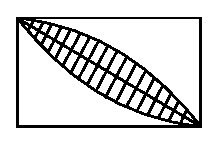
\includegraphics[scale=.95]{fig1.eps}\\
{\bf Fig. 1}
\end{figure}\pageoriginale

It is easily checked that $\varphi$ is well-defined on $S_\delta \times (0,1]$ and satisfies the conditions of the lemma.
\end{proof}

\begin{coro*}
The fundamental group at $\infty$ of $U = V - F$ is isomorphic to the fundamental group of $S_\delta$ for some (or any) $\delta < \epsilon$.
\end{coro*}

We will now examine how $S_\delta$ is built up from the $S_{\delta_i} (1 \leqq i \leqq n)$ or, what is the same, from the circle bundles $\sum_i$ associated with the normal bundles, considered as complex line bundles, of $F_i$ in $V$. For each $i$, we take the unique oriented circle bundle $\sum_i$ over $F_i \approx S^{2}$\footnote{We denote by $S^n$ the $n$-sphere, by $D^n$ the closed $n$-disc. For a subset $Y$ of a topological space $X$, we denote by $\dot{Y}$, $\bar{Y}$ and $\partial Y$ the interior, closure and boundary, respectively, of $Y$ in $X$.} of degree equal to the self-intersection number of $F_i$. If $F_i$ and $F_j$ intersect at a point $P_\alpha$, let $D^2$, $D'^2$ be closed discs of radius $\delta$ on $F_i$ and $F_j$, respectively. Denote by $\pi_i$ the projection $\sum_j \to F_i$. We have orientation-preserving trivialisations over the base $\pi^{-1}_i(D^2) \approx D^2 \times S^1$, $\pi^{-1}_j (D'^2) \approx D'^2 \times S^1$. We set $\sum'_i = \sum_i - (\pi^{-1}_i (D^2))^\circ$, and $\sum'_j =\sum_j - (\pi^{-1}_j (D'^2))^\circ$, so that these are manifolds with boundaries $D^2 \times S^1$, $D'^2 \times S^1$. We then identify $D^2 \times S^1$ and $D'^2 \times S^1$ by a homeomorphism carrying $\partial D^2 \times \{x\}$ onto $\{y\} \times S^1$ (any $x$, some $y$ depending on $x$) and $\{x\} \times S^1$ onto $\partial D'^2 \times \{y\}$ (any $x$, some $y$), preserving  orientations. If we perform this operation for all the points of intersection of different components of $F$, we end up with $S_\delta$.

Thus, we see that $S_\delta$ is determined topologically by the following data: the number of components of $F$, the pairs among them which intersect, and their self-intersection numbers; in other words, the weighted graph associated with $F$.

Note that to any subsystem $G = \{G_1,G_2, \ldots, G_m\}$ of curves of $F = \{ F_1, \ldots, F_n \}$, there corresponds a sub-graph $\Gamma'$ of $\Gamma$ such that two vertices of $\Gamma'$ are\pageoriginale linked in $\Gamma'$ if and only if they are linked in $\Gamma$, and conversely, to any such sub-graph $\Gamma'$, there corresponds a sub-system of curves of $F$.

We introduce some definitions. Let $\Gamma$ be any connected graph, and $f$ a vertex of $\Gamma$. The connected components of the graph obtained by removing $f$ from the vertices of $\Gamma$ and deleting the links at $f$ are called the branches of $\Gamma$ at $f$. We say that $f$ is a branch point if the number of branches at $f$ is at least three. Now suppose $\Gamma$ is a graph with weights $\{w_e\}$ which are real numbers attached to the vertices $\{e\}$ of $\Gamma$. On the real vector space $L (\Gamma)$ with the vertices of $\Gamma$ as basis, we introduce a symmetric bilinear form $Q = Q(\Gamma)$ by defining
\begin{center}
$Q (e, e) = w _e$  \hspace{2cm} for any vertex $e$ of $\Gamma$,
\begin{equation*}
Q (e,f) = 
\left\{
\begin{tabular}[c]{lr}
1 & \quad if $e$ and $f$ are distinct vertices linked in $\Gamma$\\
0 & \quad if $e$ and $f$ are distinct vertices not linked in $\Gamma$.
\end{tabular}
\right.
\end{equation*}
\end{center}
Note that when $\Gamma$ is the weighted graph arising from a pair $(V,F)$ as above, $Q$ is nothing but the intersection form.

\begin{lem}\label{art8-lem2}%% 2
Let $\Gamma$ be a graph with real weights $\{w_e\}$ attached to the vertices $\{e\}$  of~ $\Gamma$. Let $e$, $e'$ be two vertices of~ $\Gamma$ such that there is a unique link $\bar{ee'}$ through $e$ in $\Gamma$. Suppose $w_e \neq 0$. Let $\Gamma'$ be the graph with the same vertices as $\Gamma$, but with the link $\bar{ee'}$ omitted from the links of $\Gamma$. Define weights $\{w'_f\}$ on the vertices $\{f\}$ of $\Gamma'$ by
\begin{align*}
w'_f &  = w_f \text{ ~~if~~ } f \neq e',\\
w'_{e'} & = w_{e'} - w^{-1}_{e}.
\end{align*}
Then the quadratic forms $Q (\Gamma)$ and $Q(\Gamma')$ are equivalent by a unimodular linear transformation. In particular, they have the same discriminant (with respect to the basis consisting of the vertices of $\Gamma$).
\end{lem}

\begin{proof}
Express $Q(\Gamma)$ in terms of the basis of $L(\Gamma)$ given by 
$$
e, e' - w^{-1}_e e, f (f \neq e, e').
$$
\vskip -1cm
\end{proof}

\begin{coro*}
The determinant of the following graph with real weights $w_i$
\begin{figure}[H]
\hfill
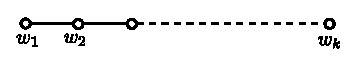
\includegraphics{fig2.eps}\hfill \raisebox{10pt}{$(k \geqq 1)$}
\end{figure}
\noindent
satisfying $w_1 < -1$, $w_i \leqq -2$ for $i > 1$, is greater than one in absolute value.
\end{coro*}

\begin{proof}
Successive applications of the lemma, starting from the left, show that the discriminant equals $\prod^k_1 q_i$, where $q_1 = w_1$, $q_{i+1} = w_{i+1} - q^{-1}_i$, Since $q_i < -1$, the result follows.

We shall denote the discriminant of $Q(\Gamma)$ by $d(\Gamma)$ and we shall write $d(F)$ for $d (\Gamma (Y, F))$.
\end{proof}

\begin{lem}\label{art8-lem3}%%% 3
Let $(V, F)$\pageoriginale be a pair satisfying conditions (i)-(vii). Then $d(F) \neq 0$ if and only if $H_i (S_\delta (F))$ is finite for small $\delta$, and in that case, $d(F)$ equals the order of $H_1 (S_\delta (F))$.
\end{lem}

\begin{proof}
We have the following commutative diagram 
{\fontsize{9}{11}\selectfont
\[
\xymatrix@C=.5cm@R=.5cm{
& H_2 (V_\delta (F)) & H^2_c (V_\delta (F)) \ar[dd] \ar[l]_-{\displaystyle\mathop\sim^{P_1}} \approx  H^2 (\bar{V}_\delta (F), S_\delta (F))  \ar[r] & H^2 (\bar{V}_\delta(F)) \displaystyle{\mathop{\approx}^\beta} H^2 (F)\\
H_2 (F) \ar[ur]^{\displaystyle\mathop\sim^\alpha} \ar[dr] & & &\\
& H_2 (V) & H^2 (V) \ar[l]_{\displaystyle\mathop\sim^{P_2}} \ar[uur] &  
}
\]}\relax

Here, $P_1$, $P_2$ are the isomorphisms of Poincar\'e duality theory, obtained by forming cap products with the fundamental classes of $V_\delta (F)$ (in the homology group of locally finite chains) and $V$, respectively, and $\alpha$ and $\beta$ are isomorphisms since $F \hookrightarrow V_\delta (F) \hookrightarrow \bar{V}_\delta (F)$ are homotopy equivalences. It follows that the composite map $H_2 (F) \to H^2 (F)$ obtained by following the upper row is that given by the intersection product $H_2 (F) \times H_2 (F) \to Z$. Hence, $d(F) \neq 0$ if and only if this pairing is non-degenerate over $Q$, and in this case $d(F)$ equals the order of the cokernel of $H_2 (F) \to H^2 (F)$, i.e., the order of the cokernel of $H^2 (\bar{V}_\delta (F), S_\delta (F)) \to H^2 (\bar{V}_\delta (F))$. Now
$$
H^3 (\bar{V}_\delta (F), S_\delta (F)) \approx H^3_c (V_\delta (F)) \approx H_1 (V_\delta (F)) \approx H_1 (F) = 0, 
$$
so that the sequence
$$
H^2 (\bar{V}_\delta (F), S_\delta (F)) \to H^2 (\bar{V}_\delta (F)) \to H^2 (S_\delta (F)) \to 0
$$
is exact. Further, by Poincar\'e duality on $S_\delta (F)$, $H^2 (S_\delta (F)) \approx H_1 (S_\delta (F))$. This proves the lemma.
\end{proof}

Now, let $(V,F)$ satisfy conditions (i)-(vii) and let $\Gamma$ be its graph. For any connected subgraph $\Gamma'$ of $\Gamma$ such that two vertices of $\Gamma'$ are linked in $\Gamma'$ if and only if they are linked in $\Gamma$, let $F''$ denote the corresponding subsystem of curves of $F$. We shall denote by $\pi (\Gamma')$ the fundamental group $\pi_1 (S_\delta (F'))$ for small $\delta$. Note that this is the fundamental group at infinity of $V - F'$. In particular, if $(W,G)$ is another pair satisfying (i)-(vii) such that $V -F$ and $W - G$ are isomorphic varieties, $\pi_1 (S_\delta (F)) \approx \pi_1 (S_\delta (G))$.


\begin{lem}[{\cite{art8-key2}Mumford}]\label{art8-lem4}%%% 4
Let $(V,F)$ satisfy (i)-(vii), and let $\Gamma$ be its graph. Let $e$ be a vertex of $\Gamma$ and $\Gamma_1, \ldots, \Gamma_p$ the branches at $e$. If $\pi(\Gamma) = (e)$, there are at most two branches $\Gamma_i$ such that $\pi(\Gamma_i) \neq (e)$.
\end{lem}

\begin{proof}
Let $G_i$ be the system of curves corresponding to $\Gamma_i$, and $G$ the component of $F$ corresponding to $e$. Then $S_\delta (F)$ is obtained as follows. From each\pageoriginale $S_\delta (G_i)$, one removes an open solid torus $(D^2_i \times S^1)^\circ$. Let $\pi: \sum (G) \to G$ be the oriented circle bundle over $G$ of degree equal to the self-intersection number of $G$. Then one removes from $\sum (G)$ certain open solid tori of the form $\pi^{-1} (D'^2_i)^\circ, D'^2_i$ being disjoint discs on $G$. Choose trivialisation of $\sum (G)$ over the $D'^2_i$ preserving orientation: $\pi^{-1} (D'^2_i) \displaystyle\mathop\approx^{\lambda_i} D'^2_i \times S^1$. Now one identifies $\partial D^2_i \times S^1$ and $\lambda^{-1}_i (\partial D'^2_i \times S^1)$ by a homeomorphism $\varphi_i$ such that $\lambda_i \circ \varphi_i$ takes circles of the form $\partial D^2_i \times \{ x\}$ onto circles of the form $\{y\} \times S^1$.

{\tolerance=1000 \parfillskip 0pt plus 0pt minus 0pt
Choose an open subset $U$ of $G$ containing all the $D'_i$ with a homeomorphism $U \approx R^2$ taking the $D_i$ onto discs in $\bfR^2$  with centers on the unit circle and small radius, such that the centers of $D'^2_1, D'^2_2, \ldots$ occur in cyclic order on the unit circle (see Fig. 2). Join the origin $O$ of $\bfR^2$ to points $x_i$ of $\partial D'^2_i$ by straight lines $l_i$. Since the fibration $\pi$ restricted to $U$ is trivial, we can choose a base point\par}


\begin{figure}[H]
\centering
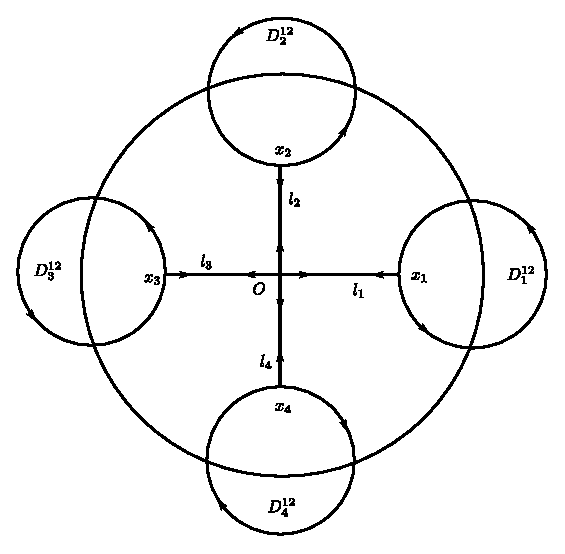
\includegraphics{fig3.eps}\\
{\bf Fig. 2}
\end{figure}

\noindent
$O'$ in\pageoriginale $\sum (G) - \cup_i \pi^{-1} (D'^2_i)$, curves $l'_i$ lifting $l_i$ leading from $O'$ to a point $x'_i$ lying over $x_i$ and loops $\gamma'_i$ at $x'_i$ whose projection $\pi (\gamma'_i)$ is the loop $\partial D'^2_i$ oriented positively at $x_i$. Finally let $\delta_i$ be the loop at $x'_i$ describing the fiber $\pi^{-1} (x_i) \approx S^1$ once positively.

The fundamental group $H$ of $\sum (G) - \bigcup_i\pi^{-1} (D'^2_i)^\circ$ is generated by $c_i = l'_i \gamma'_i l'^{-1}_{i}$, $d_i = l'_i \delta_i l'^{-1}_i$ with the relations $d_1 = d_2 = \ldots = d_p (=d, \text{ say})$, $c_i d_j c^{-1}_i d^{-1}_j =e$ and $c_1 c_2 \ldots c_p = d^r$ for some $r \in \bfZ$. Let $G'_i$ be the fundamental group of $S_\delta (G_i) - (D^2_i \times S^1)^\circ$ based at the point $y_i$ corresponding to the point $x'_i$ on $\pi^{-1} (\partial D'^2_i)$. By van-Kampen's theorem, $\pi_1 (S_\delta (G_i)) = G''_i$ is the quotient of $G'_i$ by the normal subgroup generated by the loop $\partial D^2_i \times x_i$ (for some point $x_i \in S^1$) through $y_i$. Again by van-Kampen's theorem, the fundamental group $\pi (\Gamma)$ of $S_\delta (F)$ is the quotient of the free product
$$
G'_1 * G'_2 * \ldots * G'_p * H
$$
by the normal subgroup generated by $d_i (\partial D^2_i \times x_i)^{-1} (1\leqq i \leqq p)$ and $c_i \xi'^{-1}_i$ for some $\xi'_i \in G'_i$. On dividing each $G_i$ by $\partial D^2_i \times x_i$ and $H$ by the (central) subgroup generated by $d$, we see that $\pi (\Gamma)$ has as quotient the group
$$
G''_1 * G''_2 * \ldots * G''_p / \{\xi_1 \ldots \xi_p\}
$$
where $\xi_i$ are the images of $\xi'_i$ in $G''_i$, and for any $\eta$, we denote by $\{\eta\}$ the normal subgroup generated by $\eta$.

Now, if there are three indices $i$ for which $G''_i$ is non-trivial, $\pi(\Gamma)$ has as quotient a group of the form
$$
H_1 * H_2 * H_3 /\{\eta_1 \eta_2 \eta_3\}
$$
where $H_i$ are non-trivial groups and $\eta_i \in H_i$. Since $\pi_1 (\Gamma) = \{e\}$ by the assumption, the above group should also be trivial. But by Mumford's lemma \cite{art8-key2} this group is non-trivial, which is a contradiction.
\end{proof}

\begin{lem}\label{art8-lem5}%%% 5
Let $(V,F)$ be a pair satisfying (i)-(vii) with graph $\Gamma$. Suppose there is a subgraph $\Gamma'$ of the form
\begin{figure}[H]
\hfill
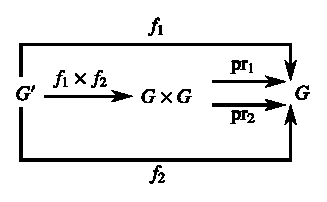
\includegraphics{fig4.eps} \hfill \raisebox{10pt}{$(k \geqq 1)$}
\end{figure}
\noindent
(where the $w_i$ denote the weights) with $\pi (\Gamma') = (e)$ such that no vertex of $\Gamma'$ is a branch point of $\Gamma$. Then there is a pair $(W,G)$ satisfying (i)-(v) and (vii) such that the following conditions hold:
\begin{itemize}
\item[(i)] There is an isomorphism of varieties $V - F \approx W - G$;

\item[(ii)] The graph of $(W,G)$ is obtained from the graph $\Gamma$ of $(V,F)$ by pinching $\Gamma'$ to a single vertex in $\Gamma$ and giving it a weight $+1$. (The weights at vertices not in $\Gamma'$ may get changed.)
\end{itemize}
\end{lem}

\begin{proof}
We proceed by induction on $k$. When $k=1$, $w_1= \pm 1$ since $\pi (\Gamma') = (e)$, and\pageoriginale $w_1 = -1$ is ruled out by assumption (vi). Assume that the result holds when the number of vertices in $\Gamma'$ is $<k$. Now, all the weights $w_i$ cannot be $<0$, since they would then be $\leqq -2$ and $|d (\Gamma')|>1$. If there are at least three non-negative weights, some two vertices which are not linked must have non-negative weights, and there is a two dimensional subspace of $L(\Gamma)$ on which $Q (\Gamma)$ is positive semi-definite. Hence the number of non-negative weights is either one or two, and if it is two, the corresponding vertices must be linked and one of the weights must be 0.

Suppose the number of non-negative weights is one, say $w_{i_0} \geqq 0$ and $w_i \leqq -2$ for $i \neq i_0$. By Lemma \ref{art8-lem2}, the discriminant $d(\Gamma')$ equals
$$
d (\Gamma') = q_1 \cdot q_2 \ldots q_{i_0-1}\cdot r_1 \cdot r_2 \ldots r_{k-i_0} \qquad (w_{i_0} - q^{-1}_{i_0-1} - r^{-1}_{k-i_0})
$$
where $q_1 = w_1$, $q_{i+1} = w_{i+1} - q^{-1}_{i}$ for $i \geqq 1$, $r_1 = w_k$, $r_{i-1} = w_{k-i+2} - r^{-1}_i$ for $i \leqq k$. (Omit the $q$'s if $i_0 = 0$ and the $r$'s if $i_0=k$). Thus, $q_i$, $r_i < -1$ and if $w_{i_0} \geqq 1$, $|d(\Gamma')|>1$. Thus, $w_{i_0} =0$, and 
$$
d(\Gamma') = - q_1 \cdots q_{i_0-2} \cdot r_1 \cdots r_{k-i_0} - q_1 \cdots q_{i_0-1} \cdot r_1 \cdots r_{k-i_0-1}
$$
if $2\leqq i_0 \leqq k -1$. This again leads to $|d(\Gamma')|>1$. Thus, $i_0$ must be 1 or $k$, and we may assume $i_0=1$ by symmetry. Again, one sees that necessarilly $k=2$, so that $\Gamma'$ has to be the weighted graph
\begin{figure}[H]
\centering
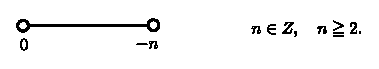
\includegraphics{fig5.eps}
\end{figure}
\noindent
Let $L$ be the line corresponding to the first vertex. If this vertex is linked to a vertex  $f$ of $\Gamma$ not in $\Gamma'$, let $L'$ be the line corresponding to $f$. Choose an arbitrary point $P$ on $L$ if there is no such $f$, and choose $P$ to be the point of intersection of $L$ and $L'$ if there is an $f$. Blow up $P$, and contract the proper transform of $L$. Repeat this procedure $(n-1)$ times, till we get a pair ($W'$, $G'$), satisfying conditions (i)-(v) and (vii) such that $V -F \approx W' - G'$, and the graph of $(W',G')$ is isomorphic to $\Gamma$. Further, the weights of $\Gamma'$ are 0 and $-1$ respectively. Contract the line corresponding to the weight $-1$, to get $(W,G)$ as required.

Next suppose there are two non-negative weights in $\Gamma'$. By condition (vii), these must be linked and one of them must be $0$. Thus, $\Gamma'$ looks like
\begin{figure}[H]
\centering
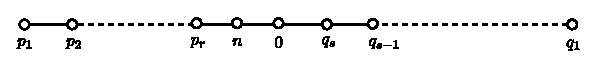
\includegraphics{fig6.eps}
\end{figure}
\noindent
with $r \geqq 0$, $s \geqq 0$, $n \geqq 0$, $r + s + 2 = k$. Blow up the point of intersection of the lines corresponding to the vertices with weights $n$ and $0$, and contract the proper transform of the line corresponding to the vertex of weight 0. Repeat this $n+1$ times to get $(W',G')$ satisfying conditions (i)-(v) and (vii) with a graph isomorphic to the original graph but the weights changed as follows:
\begin{figure}[H]
\centering
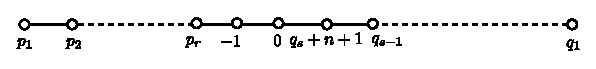
\includegraphics{fig7.eps}
\end{figure}\pageoriginale
\noindent
Now shrink the line corresponding to the vertex with weight $-1$. We get a pair $(W'',G'')$ satisfying (i)-(v) and (vii). The graph of this pair is obtained  from $\Gamma$ by pinching two adjacent vertices to one and replacing the weights $p_r$ and $0$ by $p_r+1$ and $1$, respectively. Since $k$ is now decreased, the assertion of the lemma follows by induction hypothesis.
\end{proof}

\begin{remarks*}
\begin{itemize}
\item[(1)] The pair $(W, G)$ obtained from the lemma need not necessarily satisfy (vi), since certain weights at vertices of $\Gamma$ not in $\Gamma'$ are also altered. However, the only weights which are altered are those at vertices directly linked to the first or last vertex of $\Gamma'$. Now, we can shrink suitable exceptional curves of the first kind successively to obtain a pair $(\bar{W}, \bar{G})$ which satisfies all the conditions (i)-(vii), with $\bar{W}- \bar{G} \approx V - F$. However, the graph of $(\bar W, \bar G)$ is not describable in such a simple fashion as that of $(W, G)$, though we can make the following assertion. {\em The number of branch points of the graph of $(\bar{W},\bar{G})$ is the same as that of $\Gamma$}. In fact, if this were not so, we would necessarily have (a) the maximal linear subgraph $\Gamma''$ of $\Gamma$ containing $\Gamma'$ but not any branch point of $\Gamma$ must be linked to exactly one vertex of $\Gamma$ so that it is a branch at a branch point of $\Gamma$, and (b) the system of curves corresponding to $\Gamma''$ must be collapsible to a single point on a non-singular surface. But now (b) implies that the restriction of the intersection form to the space spanned by the vertices of $\Gamma''$ is negative definite. This is not so on $\Gamma'$, as we have shown above.

\item[(2)] During the course of the proof, we have also established that there is no system of curves satisfying (i)-(vii) whose graph is linear, contains no non-negative weights, and has discriminant $\pm 1$; and that the only systems satisfying (i)-(vii) with a linear graph of discriminant 1 in absolute value containing a unique vertex with non-negative weight are those with the graphs 
\begin{figure}[H]
\centering 
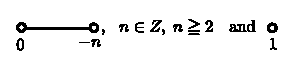
\includegraphics{fig8.eps}\raisebox{8pt} . 
\end{figure}

\end{itemize}
\end{remarks*}

\begin{lem}\label{art8-lem6}%%% 6
On a complete non-singular surface $V$ with $H^1 (V, \mathscr{O}_v) =0$, there cannot exist a system of five lines $L_i (1 \leqq i \leqq 5)$ satisfying conditions (i)-(v) whose weighted graph looks like
\begin{figure}[H]
\centering
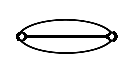
\includegraphics{fig9.eps}
\end{figure}
\noindent
with $(L^2_3) = -1 $ and $(L^2_5) \geqq 0$.
\end{lem}

\begin{proof}
Shrink $L_3$ on $V$ to a point on a non-singular surface $V'$ and denote by $L'_i (i \neq 3)$ the image of $L_i$ in $V'$. Then $L'_1$, $L'_2$ and $L'_4$ meet at a point $P$, and $L'_4$\pageoriginale and $L'_5$ meet transversally at a  point $Q \neq P$. Since $H^1(V',\mathscr{O}_{V'}) =0$ we have the exact sequence
$$
0 \to C = H^0 (V', \mathscr{O}_{V'}) \to H^0 (V', \mathscr{O}_{V'} (L'_5)) \to H^0 (L'_5, \mathscr{O}_{V'} (L'_5)|L'_5) \to 0.
$$
Thus the complete linear system $|L'_5|$ cuts out on $L'_5$ the complete linear system of divisors of degree $n = (L^2_5) \geqq 0$. Hence $|L'_5|$ has no base points, and since $(L'_4 \cdot L'_5) =1$, $|L'_5|$ cuts out the complete linear system of divisors of degree 1 on $L'_4$. Choose a divisors $D \in |L'_5|$ such that $D$ cuts out the point $P$ on $L'_4$. Since $(L'_5 \cdot L'_1) = (L'_5 \cdot L'_2)= 0$, $D$ must have $L'_1$ and $L'_2$ for components but not $L'_4$. But then,
$$
(L'_5 \cdot L'_4) = (D \cdot L'_4) \geqq ((L'_1 + L'_2) \cdot L'_4) \geqq 2,
$$
a contradiction.
\end{proof}

\begin{coro*}
With $V$ as in Lemma \ref{art8-lem6}, there cannot exist a system of four lines $\bar{L}_i (1 \leqq i \leqq 4)$ satisfying (i)-(v) whose graph looks like
\begin{figure}[H]
\centering
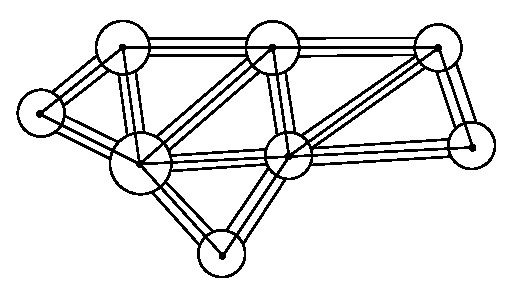
\includegraphics{fig10.eps}
\end{figure}
\noindent
and $\left(L^2_3 \right) =0$, $\left(L^2_4 \right) > 0$.
\end{coro*}

\begin{proof}
If we blow up the point of intersection of $L_3$ and $L_4$ on $V$, we are landed with a system of five lines as in Lemma \ref{art8-lem6}.

Let us call a subgraph $\Gamma'$ of a graph $\Gamma$ {\em simple} if $\Gamma'$ is linear and no vertex of $\Gamma'$ is a branch point of $\Gamma$. We shall say that a branch point of $\Gamma$ is {\em extremal} if all but one of the branches at this point are simple. We say that a connected subgraph $\Gamma'$ of $\Gamma$ is {\em spherical}\footnote{This only means that if $F'$ is the system of curves corresponding to $\Gamma'$, $S_\delta (F)$ is a homotopy 3-sphere.} if $\pi (\Gamma') = (e)$.

The proof of the main theorem follows immediately from the following 
\end{proof}

\begin{prop*}
There is no pair $(V,F)$ with $H^1 (V, \mathscr{O}_V) =0$ satisfying (i)-(vii) such that $\pi_1 (S_\delta (F)) = (e)$ and the graph $\Gamma$ not linear.
\end{prop*}

\begin{proof}
Suppose in fact that there is such a pair. By Lemma \ref{art8-lem5} and the succeeding remark (1), we may assume that any simple branch at any branch point which is spherical consists of a single vertex with weight 1. Let $k \geqq 1$ be the number of branch points of $\Gamma$.

Suppose first that $k=1$, and let $e$ be the branch point. Then the branches at $e$ are all simple; if these are $\geqq$ 4 in number, at least two of them must be spherical by Lemma \ref{art8-lem4} and hence consist of single vertices with weight 1. But this clearly contradicts (vii). Thus there are exactly three branches, and one of them\pageoriginale is spherical, hence consists of a vertex of weight 1. The graph looks like
\begin{figure}[H]
\centering
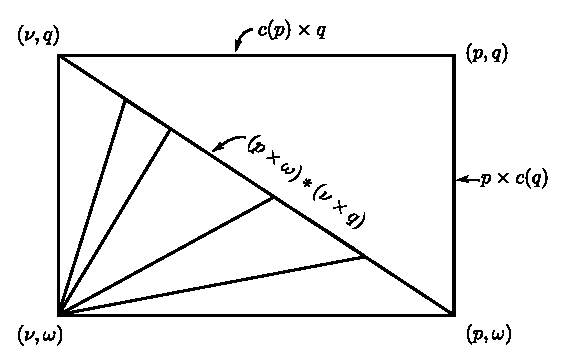
\includegraphics{fig11.eps}
\end{figure}
\noindent
where  $\Gamma_i$ are simple branches. By (vii), the weights of the vertices on $\Gamma_i$ must be $\leqq -2$, and the weight $w$ at $e$ is $\leqq 0$. If $w=0$, we get a contradiction by the Corollary to Lemma \ref{art8-lem6}. If $w \leqq -1$, use Lemma \ref{art8-lem2} to conclude that $d(\Gamma) =$ the discriminant of the graph \raisebox{-10pt}{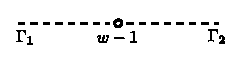
\includegraphics{fig12.eps}}, the weights in this graph at vertices on $\Gamma_i$ being the same as in the original one. Since $w -1 \leqq -2$, we see that $|d(\Gamma)|>1$ by the Corollary to Lemma \ref{art8-lem2} and we get a contradiction by Lemma \ref{art8-lem3}.

Hence suppose $k>1$, and that we have ruled out the possibility of a pair as in the proposition with fewer branch points. Let $S$ denote the set of extremal branch points of $\Gamma$. We assert that $\Card (S) \geqq 2$. In fact, start from an arbitrary branch point $e$ of $\Gamma$. We assert that $\Card (S) \geqq 2$. In fact, start from an arbitrary branch point $e$ of $\Gamma$. There is a branch at $e$ containing a branch point of $\Gamma$, since $k  \geqq 2$, and there are at least two such branches at $e$ if $e$ is not extremal. Travel along one of these branches (without retracting one's path) till one reaches a branch point $f$. If $f$ is not extremal, we can choose a branch at $f$ not containing $e$ but containing a branch point. Travel along this branch. Continuing in this manner, we see that on every branch at $e$ which is not simple, there is an extremal branch point. This proves that $\Card (S) \geqq 2$.

Denote by $S'$ the subset of $S$ consisting of those vertices $e \in S$ such  that every simple branch at $e$ carries only weights $<0$ (hence $\leqq -2$). Because of (vii), we have $\Card (S')\geq \Card (S) -1 \geqq 1$.

Let $e$ be an arbitrary element of $S'$. There must be exactly two simple branches at $e$, since otherwise there would exist a simple spherical branch at $e$ by Lemma \ref{art8-lem4} and this branch would consist of a single vertex with weight 1 by assumption, contradicting the fact that $e \in S'$. Let $\Gamma'$ be the non-simple spherical branch at $e$ and $f$ the point of this branch linked to $e$ in $\Gamma$. If $f$ is a branch point of $\Gamma'$, the system of curves corresponding to $\Gamma'$ would satisfy (i)-(vii) and $\Gamma'$ is spherical, which is impossible by the induction hypothesis. For the same reason, it cannot happen that $f$ is not a branch point of $\Gamma$. Thus $f$ is a branch point of $\Gamma$ with exactly three branches in $\Gamma$ at $f$.

We deal separately with the case $k=2$. The graph looks like
\begin{figure}[H]
\centering
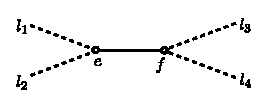
\includegraphics{fig13.eps}
\end{figure}
where $e$ and $f$ are linked branch points and $l_i (1 \leqq i \leqq 4)$ are simple branches such that the weights on $l_1$, $l_2$ and one of $l_3$, $l_4$, say $l_3$, are negative. Let $\delta_i$ be the\pageoriginale discriminants of $l_i$ and $\Delta_1$ and $\Delta_2$ the discriminants of \raisebox{-7pt}{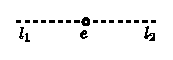
\includegraphics{fig14.eps}} ~and~ \raisebox{-9pt}{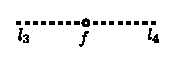
\includegraphics{fig15.eps}} respectively. By taking the weights to be variables and applying Lemma \ref{art8-lem2} repeatedly to remove the links on the simple branches and the links connecting these branches to the branch points, one obtains the identity $\disc (\Gamma) = \Delta_1 \Delta_2 - \delta_1 \delta_2 \delta_3\delta_4$. Since \raisebox{-7pt}{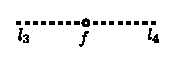
\includegraphics{fig15.eps}} is spherical, $|\Delta_2|=1$, and since the weights on $l_i(1 \leqq i \leqq 3)$ are $\leqq - 2$, $|\delta_i| >1$ and hence $\geqq 2$ by the Corollary to Lemma \ref{art8-lem2}. If $\delta_4 =0$, the quadratic form of $l_4$ is degenerate, and hence by (vii) should be negative semi-definite with null-space of dimension one. If this happens, there must be a non-negative weight in $l_4$ and this weight must then necessarily be  0. The corresponding vertex must belong to the null-space of the quadratic form. But then, this vertex cannot be linked to any other vertex of $l_4$, so that $l_4$ should reduce to a single vertex with weight 0. But then, the graph $l_1 el_2$ cannot be spherical, since we would then have $w_e = -1$ by remark (2) following Lemma \ref{art8-lem5}, in contradiction to Lemma \ref{art8-lem6}. Suppose then that $\delta_4 \neq 0$, so that $|\delta_4| \geqq 1$ and $|\delta_1 \delta_2 \delta_3 \delta_4| \geqq  8$; since $1 = |d(\Gamma)| =|\Delta_1 \Delta_2 - \delta_1 \delta_2 \delta_3 \delta_4|$ and $|\Delta_2| =1$, we must have $|\Delta_1| \neq 1$ and again $l_1 el_2$ cannot be spherical. Applying Lemma \ref{art8-lem4} to the branch point $f$, we deduce that $l_4$ is spherical, hence reduces to a single vertex with weight 1. Because of (vii) we must have $w_f \leqq 0$, and by the Corollary to Lemma \ref{art8-lem6}, $w_f \neq 0$, so that $w_f \leqq -1$. Using Lemma \ref{art8-lem2}, the discriminant of $l_3 f l_4$ equals that of $l_3 f$ with $w_f$ replaced by $w_f -1$, so that all the weights of the latter graph are $\leqq - 2$ and its discriminant exceeds 1 in absolute value, a contradiction.

Thus, we assume from now on that $k \geqq 3$. Reverting to our old notations, we have seen that if $e \in S'$, there are two simple branches at $e$, and on the third spherical branch $\Gamma'$, the point $f$ linked to $e$ is a branch point of $\Gamma$ with three branches. Since $\Gamma'$ has at least one branch point, if $w_f \neq -1$, the system of curves corresponding to $\Gamma'$ satisfies conditions (i)-(vii) and $\Gamma'$ is spherical, which is impossible by the induction hypothesis. Furthermore, $\Gamma'$ satisfies conditions (i)-(v) and (vii), and (vi) can be ensured by successively contracting exceptional curves corresponding to non-branch points. Since $\Gamma'$ is spherical, this implies that the above process of shrinking suitable exceptional curves should eliminate all branchings. As is easily seen, this implies in paricular that one of the branches at $f$ is simple with all weights less than, 0, hence $\leqq -2$. Thus, in the vicinity of a point $e \in S'$, $\Gamma$ looks like 
\begin{figure}[H]
\hfill
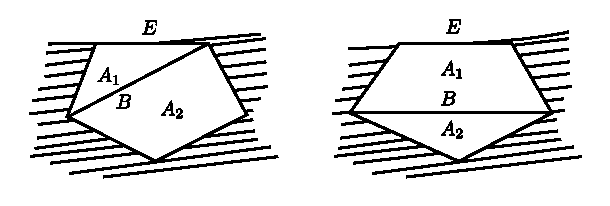
\includegraphics{fig16.eps}\hfill \raisebox{10pt}{$(e \in S')$}
\end{figure}
\noindent
where\pageoriginale the $l_i$ are simple branches, all having weights $\leqq -2$, $w_f = -1$, and $\gamma$ is an arbitrary branch containing at least one branch point of $\Gamma$.

Define $S'' = \{e \in S' | w_e = -1\}$. Suppose $S'' \neq \varnothing$; then the intersection form is 0 on $e+f$. We assert that this implies that there is no non-negative weight. In fact, if $w_g \geqq 0$ for some $g$, then by condition (vii), $g$ must be linked to either $e$ or $f$. But this is again impossible by Lemma \ref{art8-lem6}. In particular, we have $S = S'$. Suppose on the other hand that $e \in S' - S''$. Then $l_1 el_2$ cannot be spherical by the Corollary to Lemma \ref{art8-lem5} and the remarks following it. Thus, Lemma \ref{art8-lem4} applied to $f$ gives us that $\gamma$ is spherical. Since $\gamma$ contains branch points of $\Gamma$, we deduce as before that the point on $\gamma$ linked to $f$ is a branch point of $\Gamma$ with exactly three branches.

Let us dispose of the case $k=3$. Suppose first that $S'' \neq \varnothing $ and $e \in S''$. Denote by $g$ the third branch point besides $e$ and $f$. We know that all weights are $<0$. Suppose $g$ is not linked to $f$ directly. We can then apply Lemma \ref{art8-lem4} to $\Gamma$ at $g$ to get a contradiction to our induction hypothesis. By the same token, there are exactly three branches at $g$, two of them simple. Now, we know that $\Gamma'$ is spherical. Apply Lemma \ref{art8-lem4} to $\Gamma'$ at $g$ to deduce that all the weights on $l_3$ equal $-2$. Apply Lemma \ref{art8-lem4} to $\Gamma$ at $g$ to deduce that 
\begin{figure}[H]
\centering
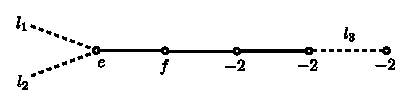
\includegraphics{fig17.eps}
\end{figure}
\noindent
is spherical. Note that $w_e = w_f = -1$. Shrink the curves corresponding to vertices on the branch at $e$ containing $l_3$, to get a linear spherical graph with all but one of the weights $\leqq -2$ and a weight at a unique vertex which is not an end vertex $\geqq 0 $. This is impossible. Thus, $S'' = \varnothing$, and in this case, by what we have seen earlier, the graph looks like
\begin{figure}[H]
\centering
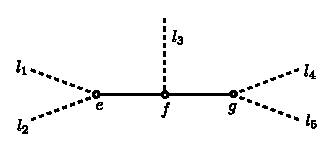
\includegraphics{fig18.eps}
\end{figure}
\noindent
with all the weights on $l_1$, $l_2$ and $l_3$ and one of $l_4$ or $l_5$, say $l_4$, negative, and $w_f = -1$, $w_e \neq -1$. Now, $l_5$ cannot be spherical since it would then consist of a single vertex of weight 1 by assumption, contradicting Lemma \ref{art8-lem6}. Applying Lemma \ref{art8-lem4} at $g$, we see that 
\begin{figure}[H]
\centering
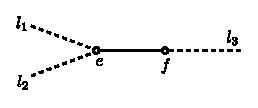
\includegraphics{fig19.eps}
\end{figure}
\noindent
is spherical. Thus the horizontal branch of this graph at $e$ should be collapsible, and all the weights on $l_3$ should be equal to $-2$. Now, both the graphs
\begin{figure}[H]
\centering
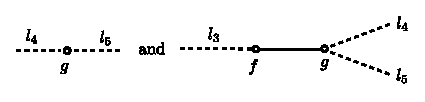
\includegraphics{fig20.eps}
\end{figure}\pageoriginale
\noindent
are spherical, hence have discriminants $=\pm 1$. But the discriminant of the second graph equals that of the first graph with $w_g$ replaced by $w_g+r$ where $r$ is an integer $\geqq 2$. But clearly the discriminant of the first graph is a linear function of $w_g$, the coefficient of $w_g$ being $\delta_4 \delta_5$, where $\delta_i$ is the discriminant of $l_i$. Now, $\delta_i$ are intergers, $|\delta_4| \geqq 2$, so that the above can happen only if $\delta_5=0$. But then the quadratic form of $l_5$ must be negative semi-definite with null-space of dimension one. Thus, at least one weight on $l_5$ is $\geqq 0$, hence equal to 0. This vertex must therefore belong to the null-space, and must be orthogonal to all the vertices for the quadratic form. Thus, $l_5$ consists of a single vertex of weight 0, contradicting Lemma \ref{art8-lem6}. 

Hence $k= 3$ is impossible, and we assume from now on that $k \geqq 4$. We look more closely at the branch $\gamma$ when $e \in S' - S''$. Since $\gamma$ is spherical and contains at least two branch points of $\Gamma$, one of which, say $g$, is linked to $f$, we deduce as before that $w_g = -1$ and one of the three branches at $g$ is simple with weights $\leqq -2$. Thus, in the vicinity of $e$, $\Gamma$ looks like
\begin{figure}[H]
\centering
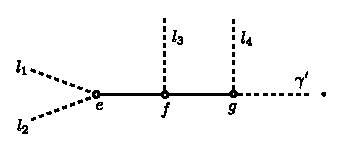
\includegraphics{fig21.eps}
\end{figure}
\noindent
Further, $\Gamma'$ spherical gives us that all the weight on $l_3$ should be $-2$. Again, a repetition of an earlier argument applied to the branch $\gamma$ tells us that there is a branch point of $\Gamma$ in $\gamma'$ linked to $g$ in $\Gamma$. But then, $\gamma$ being spherical implies that all the weights on $l_4$ equal $-2$.

Now, collapse all exceptional curves at non-branch points of $\Gamma'$, that is, collapse the branch $l_3f$ at $g$. We are left with the graph $\gamma$:
\begin{figure}[H]
\centering
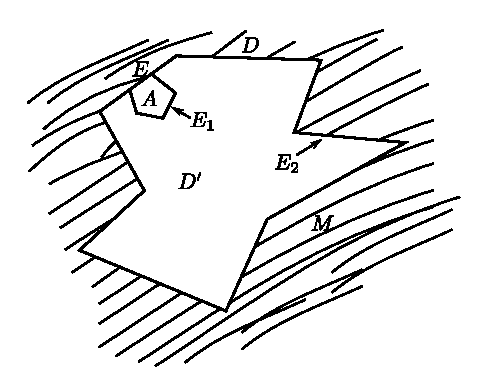
\includegraphics{fig22.eps}
\end{figure}
\noindent
except that the weight at $g$ is replaced by $w_g + r = r -1$, $r$ an integer $\geqq 2$. But this graph fulfills all the conditions (i)-(vii), contains a branch point and is spherical, which is impossible. Thus for $k \geqq 4$, $S'-S'' = \varnothing$, $S' = S''$, and hence (since $\Card (S') \geqq 1$) $S = S' = S''$, $\Card (S) \geqq 2$. Choose two distinct vertices $e$, $e' \in S''$, and denote the objects corresponding to the objects $l_i$, $f$, $\gamma$ associated to $e'$ by the same symbols with a prime. Since $e +f$ and $e'+ f'$ both have self-intersection 0, one of $e$, $f$ must either coincide with or be linked to one of $e'$, $f'$. But $e$ is linked only to $f$ besides non-branch points and $e'$ only to $f'$ besides non-branch points. Thus, either $f = f'$ or $f$ and $f'$ are linked. If $f=f'$,\pageoriginale looking at the structure of $\Gamma$ near $e$ and $e'$, we see that there can be only three branch points $e$, $f = f'$ and $e'$. Hence $f$ and $f'$ are linked, and $\Gamma$ looks like
\begin{figure}[H]
\centering
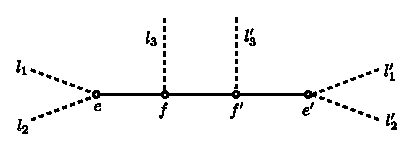
\includegraphics{fig23.eps}
\end{figure}
\noindent
with all weights $<0$, $w_e = w_{e'} = w_f = w_{f'} = -1$. Now, the fact that the non-simple branch at $e$ is spherical gives us (by our induction hypothesis) that all the weights on $l_3$ are equal to $-2$. Collapsing $l_3f$ on this branch by successively shrinking lines corresponding to non-branch vertices with weight $-1$ gives us that the graph
\begin{figure}[H]
\centering
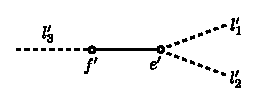
\includegraphics{fig24.eps}
\end{figure}
\noindent
where the weight at $f'$ is replaced by $w_{f'} + r = r-1$, $r \geqq 2$, is spherical. But this new graph satisfies all the conditions (i)-(vii) and contains a branch point. This is impossible.

Thus the Proposition is proved.
\end{proof}

The theorem follows almost immediately. In fact, imbed $X$ in $\bar{X}$ such that $\bar{X} - X = Y$ satisfies conditions (i)-(vii) as explained at the beginning of this section.  By the Corollary to Lemma \ref{art8-lem1} and the Proposition $\Gamma (Y)$ does not contain branch points, and is hence linear. By Lemma \ref{art8-lem5}, we may assume that $Y \approx \bfP^1$ and has self-intersection 1. The exact sequence
\begin{align*}
0 \longrightarrow \bfC = H^0 (\bar{X}, \mathscr{O}_{\bar{X}}) & \longrightarrow  H^0 (\bar{X}, \mathscr{O}_{\bar{X}} (Y))\\
& \longrightarrow H^0 (Y, \mathscr{O}_{\bar{X}} (Y)|Y) \longrightarrow  H^1 (\bar{X}, \mathscr{O}_{\bar{X}}) = 0 
\end{align*}
shows that the complete linear system $|Y|$ has no base points, and defines a morphism $\varphi$ of degree 1 (since $(Y^2) =1$) into $\bfP^2$. Since the Neron-Severi group of $\bar{X}$ is $\bfZ$, $\varphi$ cannot contract any curve, so that $\varphi$ is an isomorphism. Hence $X = \bar{X} - Y \approx \bfP^2 - \{\text{line}\} = \bfC^2$, proving the theorem.

\section{The counter-example}\label{art8-sec3}%%%%% 3

Consider in the projective plane $\bfP^2$ a cubic curve $C_1$ with a cusp and a non-degenerate conic $C_2$ meeting $C_1$ at two distinct points $P$ and $Q$, which are simple on $C_1$ and different from the inflexion point of $C_1$, with intersection numbers 5 and 1 respectively. (That such a configuration exists, and in fact, $C_1$ and either $P$ or $Q$ can be chosen arbitrarily, is easily seen, for instance using\pageoriginale the fact that $C_1$-$\{$cusp$\}$
is an algebraic group isomorphic to the additive group of $\bfC$, and a conic meets $C_1$ at simple points $P_i (1 \leqq i \leqq 6)$, each point being repeated as many times as the intersection multiplicity, if and only if $\sum^6_1 P_i = 0$ for this group law.) Blow up the point $Q$ to obtain a variety $F$ and let $C'_i$ be the proper transform of $C_i$. The veriety $X=F-C'_1-C'_2$ is our counter-example.

Put $C' = C'_1 \cup C'_2$, so that $C'$ is topologically the wedge of two 2-spheres, so that $H_1 (C') =0$ and $H_2 (C')$ is the free abelian group on the classes defined by $C'_1$ and $C'_2$. Now, $F$ is simply-connected, and $H_2 (F)$ is generated by the class $E$ of the exceptional curve and the class $H$ defined by the total transform of a line in $\bfP^2$. But in $H_2(F)$, we have the relations $C'_1 = 3 H- E$, $C'_2 = 2 H-E$. Further, $H_3 (F) \approx H^1 (F) =0$. Thus $H_i(C) \to H_i (F)$ is an isomorphism for $0 \leqq i \leqq 3$, and $H_i (F,C) =0$ for $0 \leqq i \leqq 3$. Thus we also have
$$
H_i(X) = H^{4-i}_c(X) = H^{4-i} (F,C) =0, \quad 1 \leqq i \leqq 4. 
$$
To show that $X$ is contractible, it suffices to show that $\pi_1 (X)$ is abelian, since it would then follow that $\pi_1 (X) = H_1 (X) = (e)$.

Now $F$ is a projective line bundle over $\bfP^1$ whose fibers are the proper transforms of the lines in $\bfP^2$ through the point $Q$ in $F$. Since the intersection number of any fiber with $C'_2$ is 1, $C'_2$ is a section of this fibration  $\pi: F \to \bfP^1$ and the restriction of $\pi$ to $F - C'_2$ is an affine line bundle over $\bfP^1$. If $P'$ is the inverse image of $P$, we may assume that $\pi(P)$ is the point at infinity. If $G = F - C_2 - \pi^{-1} (\infty)$, $G$ is an affine line bundle over $\bfP^1 - (\infty) = \bfC$. Since affine line bundles over $\bfC$ are trivial, we have $G \approx \bfC \times \bfC$ such that the restriction of $\pi$ to $G$ identifies itself to the first projection of $\bfC \times \bfC$ onto $\bfC$. Now, the proper transform of a line through $Q$ in $\bfP^2$ meets $C'_1$ in one point if and only if either the line passes through the singularity of $C_1$ or the line is tangent to $C_1$ at a point which is simple and distinct from $Q$. Now, it is easily seen that there is exactly one line through $Q$ tangent to $C_1$ at a simple point other than $Q$ and this point has to be distinct from $P$ or the inflexional point of $C_1$. Since $C'_1$ and $C'_2$ meet only at the point $P'$, $G \cap C'_1$ is proper over $\bfC$, of degree 2, and exactly two fibers of the map $G \cap C_1 \to \bfC$ reduce to a single point. Denoting the coordinates in $\bfC \times \bfC$ by $(z,w)$, we see that the equation of $C'_1$ in $\bfC \times \bfC$ has the form $w^2 + a(z) w - p(z) =0$, $a$, $p \in \bfC [z]$. Replacing $w$ by $w + \varphi (z)$ for a suitable polynomial $\varphi$, we may assume that the equation is $w^2 = p(z)$. Since exactly two fibers in $C'_1$ reduce to a point, $p(z)$ has exactly two zeros and after a linear change of $z$ and $w$ we may assume the equation of $C'_1$ in $\bfC \times \bfC$ has the form 
\begin{equation*}
w^2 = z^m (z-1)^n, \tag*{$m$, $ n \geqq 1$.}
\end{equation*}
 We may\pageoriginale assume that the singularity of $C'_1$ lies over 0, and the the point over 1 in $C'_1$ is simple. This gives $n=1$, and the fact that the singularity of $C'_1$ is an ordinary cusp (i.e., on blowing up the singular point, the proper transform of $C_1$ is non-singular and touches the exceptional curve exactly one point) gives us that $m=3$. Thus, $C'_1 \cap \bfC \times \bfC$ has the equation
$$
w^2 =z^3 (z-1).
$$
Now, $\bfC \times \bfC - \{z (z-1) =0\} - C'_1$ is a locally trivial fiber space over $\bfC - \{0,1\}$ with typical fiber the complex plane with two points removed. The homotopy exact sequence shows that $\pi_1 (\bfC \times \bfC - \{z (z-1) =0\} -C'_1)$ is generated by the fundamental group of the fiber and loops at the base points whose images by $\pi$ are loops around 0 and 1 in $\bfC - \{0,1\}$. Choose the base point to be $(1/2,M) = A$ with $M$ sufficiently large. Further note that 
$$
\pi_1 (\bfC \times \bfC - \{z(z-1) =0 \} - C'_1) \longrightarrow \pi_1 (\bfC \times \bfC - C_1)
$$
is surjective. We can choose loops at $A$ lifting the loops at $1/2$ in $\bfC - \{0,1\}$ around 0 and 1 with the $w$-co-ordinate constantly $M$, and these loops can be contracted in $\bfC \times \bfC - C'_1$. Thus we see that $\pi_1 (\bfC \times \bfC - C'_1)$ is generated by the fundamental group of any fiber of $\bfC \times \bfC - C'_1 \to \bfC$ over a $\lambda \in \bfC$, $\lambda \neq 0$, $1$. Since the $w$-co-ordinates of the two points of $C'_1$ lying over a $\lambda$ tend to 0 as $\lambda$ tends to 1, if $U$ is any connected neighborhood of $(1,0)$ in $\bfC \times \bfC$, $\pi_1 (U-C'_1) \to \pi_1 (\bfC \times \bfC - C'_1)$ is surjective. Now choose $U$ such that there are co-ordinates $(z',w')$ valid in $U$ and mapping it on to the polycylinder $\{ (z', w')||z'| < 1, |w'|<1\} $ such that $C'_1 \cap U$ is mapped onto $z'=0$. Then $\pi_1 (U - C'_1)$ is infinite cyclic. We have thus proved that $X$ is contractible. Now, after successive blowings up of points on $C'_1 \cup C'_2$ and its inverse images, starting from $F$, we get an embedding $X \hookrightarrow \bar{X}$ where $\bar{X}$ is a non-singular complete surface and the pair $(\bar{X},\bar{X} -X)$ satisfies conditions (i)-(vii) of \S ~\ref{art8-sec2}. The associated graph takes the form
\begin{figure}[H]
\centering
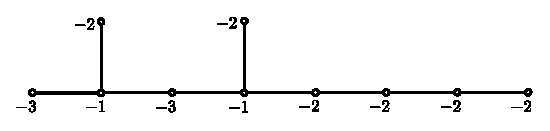
\includegraphics{fig25.eps}
\end{figure}
\noindent
This graph is not spherical, as is seen by applying Lemma \ref{art8-lem4} successively at the two branch points. On the other hand, this system of curves forms a basis for $H_2 (\bar{X})$, and hence by Poincar\'e duality over $\bfZ$, the discriminant of this graph is one in absolute value. Denoting this system of curves on $\bar{X}$ by $Y$, with the notations of \S ~\ref{art8-sec2}, we see that for small $\delta$, $\bar{X} - V_\delta (Y) = M$ is a contractible compact 4-manifold with boundary $\partial M$ a homology sphere but not a homotopy sphere.

Consider\pageoriginale the manifold $M' = M \times [0,1] \times [0,1]$ with boundary
$$
\partial M' = \partial M \times [0,1] \times [0,1] \cup M \times \{0,1\} \times [0,1] \cup M \times [0,1] \times \{0,1\}.
$$
Then $M'$ is contractible and $\partial M'$ is a homotopy sphere. By the $h$-cobordism theorem, $\partial M'$ is homeomorphic to a sphere and $M'$ to a disc. It follows from well-known theorems that $X \times \bfR^2$ is homeomorphic to $\bfR^6$.

We may thus conclude that either $X$ is an affine rational non-singular surface with $X \times \bfC$ isomorphic as an algebraic variety to $\bfC^3$ but $X$ not isomorphic to $\bfC^2$; or, that there is a non-singular affine rational variety $Y (=  X \times \bfC)$ of dimension 3 homeomorphic to $\bfC^3$ but not isomorphic to $\bfC^3$. We are unable to decide which of these possibilities holds in fact, or in other words whether $X \times \bfC \approx \bfC^3$ or not.

The author wishes to thank M. P. Murthy and C. S. Seshadri for helpful discussions. He is grateful to his sister C. P. Bhamini for her painstaking typing of the manuscript. Finally, he would like to acknowledge several suggestions for improvement of the exposition made by the referee. 

University of Warwick

\begin{thebibliography}{99}
\bibitem{art8-key1} Abhyankar,  S. S., Ramification theoretic methods in algebraic geometry. Annals Math. Studies. Princeton.

\bibitem{art8-key2} Mumford, D., The topology of normal singularities of an algebraic surface and a criterion for simplicity, Publ. Math. No 9 de l'Inst. des Hautes Etudes Sci. Paris. 

\bibitem{art8-key3} Nagata, M., {\em On embedding an abstract variety in a complete variety}, J. Math. Kyoto University 2 (1962).

\bibitem{art8-key4} Shafarevich, I. R., Lectures on the theory of minimal models. Tata Institute lecture notes in mathematics. Bombay.
\end{thebibliography}

\begin{center}
{Recived June 10, 1970}
\end{center}



